\documentclass{article}

\usepackage{titlesec}
\usepackage{amsmath}
\usepackage{amsthm}
\usepackage{amsfonts}
\usepackage{graphicx}
\usepackage{float}
\title{Numerical Methods for Ordinary Differential Equations}
\author{Murray Heymann \\
	Technische Universit{\"a}t Kaiserslautern \\
	413121}
\date{\today}

\theoremstyle{definition}
\newtheorem{theorem}{Theorem}[section]


\titleformat{\section}{\normalfont \LARGE \bfseries}
{Problem\ Sheet\ \thesection}{2.3ex plus .2ex}{}
\titleformat{\subsection}{\normalfont \Large \bfseries}
{Question\ \thesubsection}{2.3ex plus .2ex}{}
\titlespacing{\subsubsection}{2em}{*1}{*1}

\begin{document}
\maketitle


\setcounter{section}{2}
\section{}
\subsection{}

\begin{itemize}
	\item[(a)]
		As before, the function $y = e^{- \lambda t}$ was approximated.

		For stepsizes larger than $2/\lambda$, the explicit Euler method
		is not stable.  Indeed this is clearly demonstrated by the
		following graphs, using the implementation from exercise $1$.
		\begin{figure}[H]
			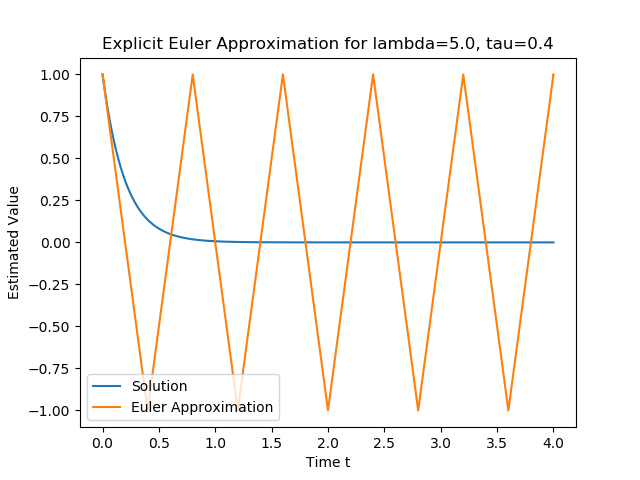
\includegraphics[scale=0.6]{explicit_euler_04}
		\end{figure}
		The approximation certainly does not
		converge to zero, but just jumps between 1 and -1.
		\begin{figure}[H]
			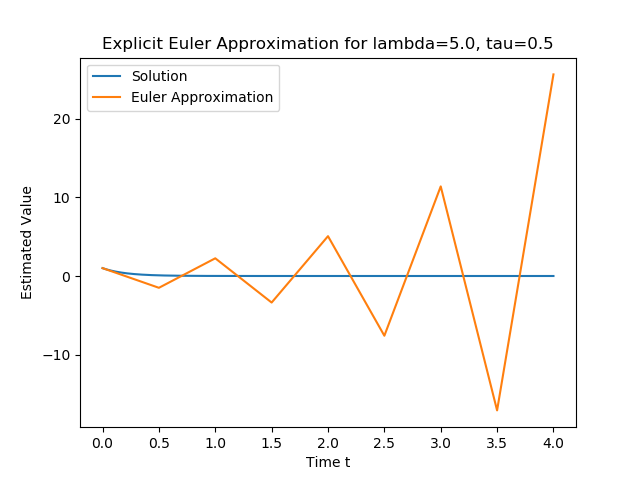
\includegraphics[scale=0.6]{explicit_euler_05}
		\end{figure}
		Here the value has no limit, while the absolute value of the
		approximation goes to infinity.

		Using a much larger $\tau = 0.6$ as stepsize, we see get the
		following approximation using
		the implicit midpoint method:
		\begin{figure}[H]
			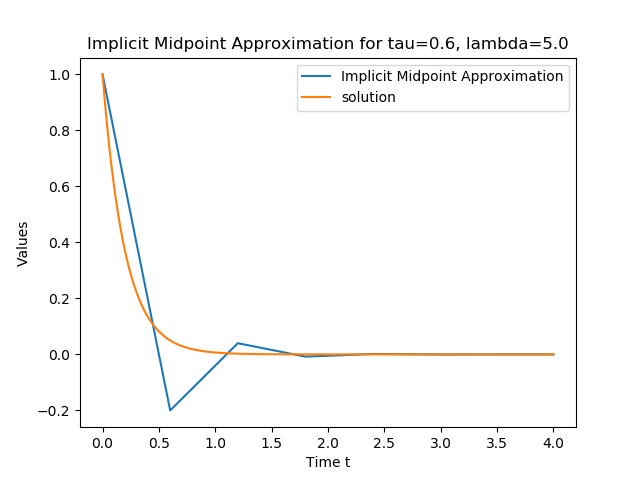
\includegraphics[scale=0.6]{implicit_mid_06}
		\end{figure}
		While it cannot be considered a good approximation in itself, it
		is noticable that the approximation is absolutely convergent to
		$0$, even though our step size is larger than in the explicit
		Euler case. For a stepsize of $\tau=0.2$, which is still
		relatively large, we get the following approximation:
		\begin{figure}[H]
			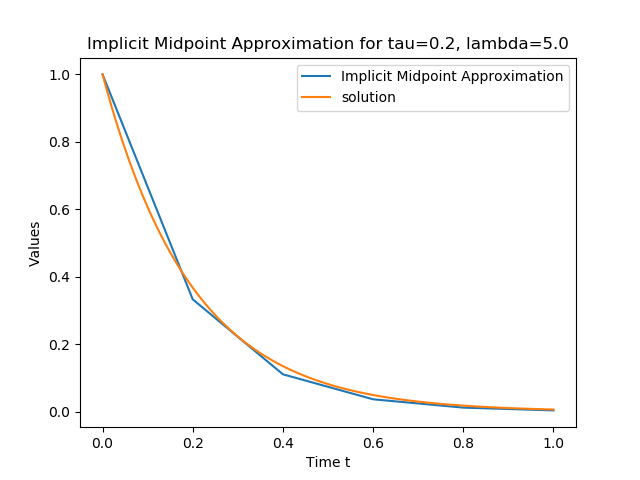
\includegraphics[scale=0.6]{implicit_mid_02}
		\end{figure}
		The local error of the implicit midpoint
		method is shown in the following log-log graph:
		\begin{figure}[H]
			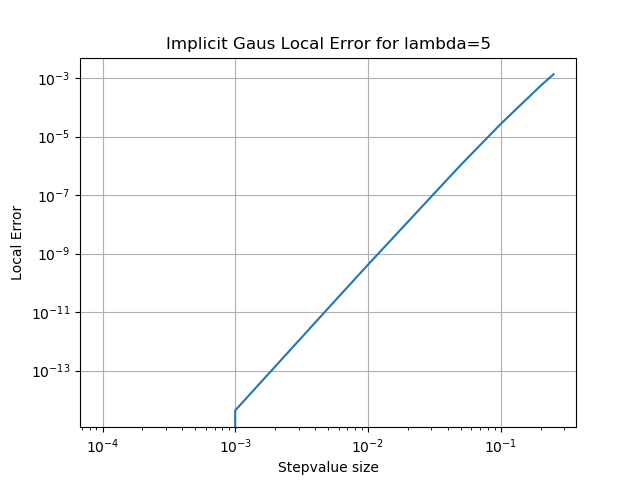
\includegraphics[scale=0.6]{implicit_gauss_local_loglog}
		\end{figure}
		The graph is a line with a gradient of about $3$, which is
		consistent with an order $2$ method.
		The global error of the implicit midpoint
		method is shown in the following log-log graph:
		\begin{figure}[H]
			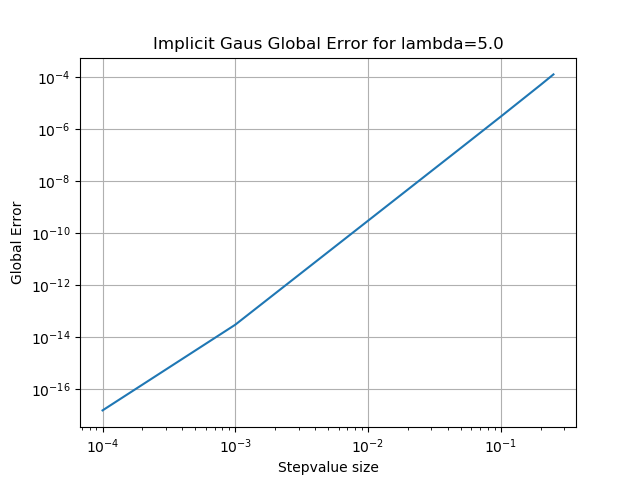
\includegraphics[scale=0.6]{implicit_gauss_global_loglog}
		\end{figure}
		It is a line with a gradient of about $2$, which confirms that
		this is an order $2$ method.

		Using $\tau = 0.6$ again as stepsize, we see get the
		following approximation using
		the implicit Gauss method:
		\begin{figure}[H]
			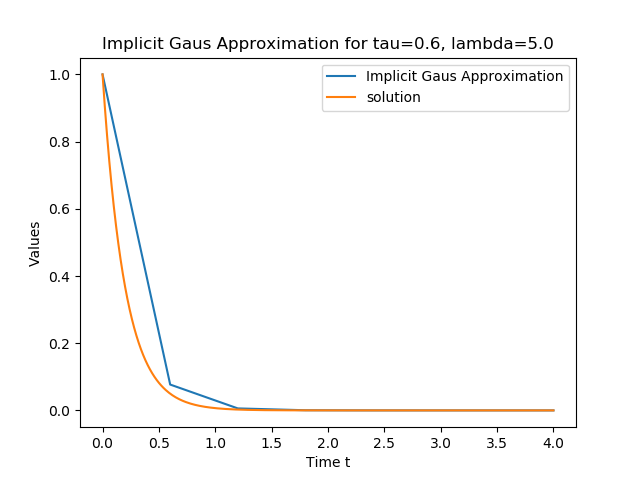
\includegraphics[scale=0.6]{implicit_gauss_06}
		\end{figure}
		It is again
		noticable that the approximation is absolutely convergent to
		$0$, even though our step size is larger than in the explicit
		Euler case. For a stepsize of $\tau=0.2$, which is still
		relatively large, we get the following approximation:
		\begin{figure}[H]
			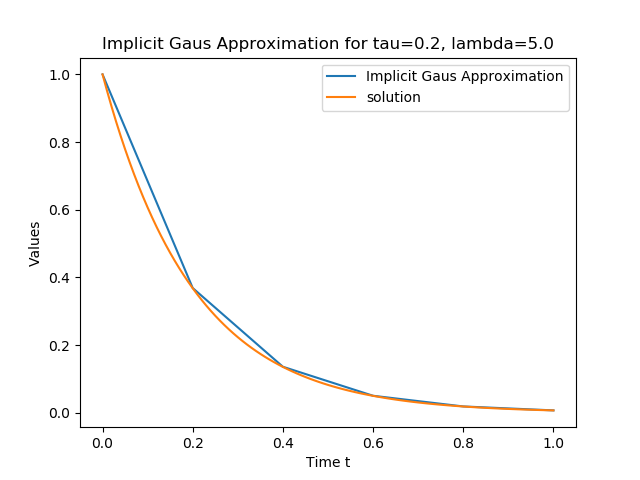
\includegraphics[scale=0.6]{implicit_gauss_02}
		\end{figure}
		The local error of the implicit Gauss
		method is shown in the following log-log graph:
		\begin{figure}[H]
			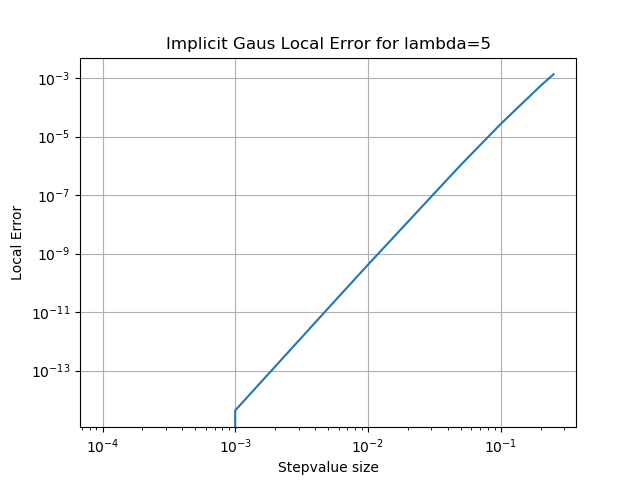
\includegraphics[scale=0.6]{implicit_gauss_local_loglog}
		\end{figure}
		The graph is a line with a gradient of about $5$, which is
		consistent with an order $4$ method.  It should be noted that
		for stepsizes less than $0.001$, the local error was calculated
		as $0$.  This does not mean that there is no error, simply that
		the error was smaller than the implementation can represent as a
		floating point number.
		The global error of the implicit midpoint
		method is shown in the following log-log graph:
		\begin{figure}[H]
			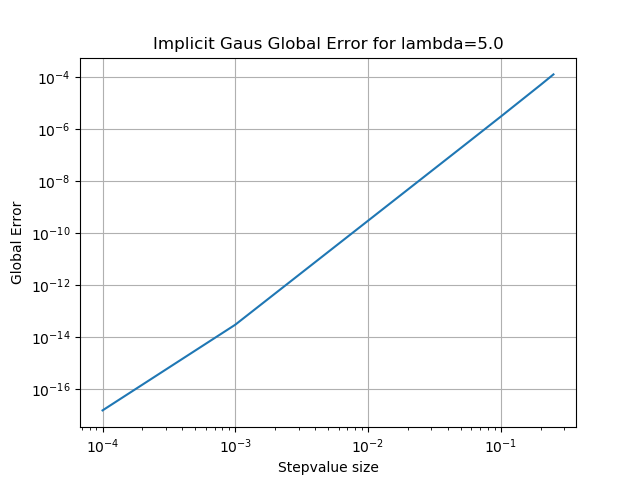
\includegraphics[scale=0.6]{implicit_gauss_global_loglog}
		\end{figure}
		It is a line with a gradient of about $4$, which confirms that
		this is an order $4$ method. For very small stepsizes, the error
		seems to no longer descend along the same curve.  This is most
		likely because of the additional error introduced by Newton's
		method for approximating the $\mathbf{k}_i$'s in the implicit Runge-Kutta
		method.


	\item[(b)]
		First, let's discuss norm preserving linear continuous
		evolutions.
		We have already seen in Theorem 4.27 that if the $A$ is
		skew-symmetric, then $e^{tA}$ is an orthogonal, and hence norm
		preserving. It so happens
		that the converse is also true.

		\begin{theorem} \label{norm_preserving_skew_symmetric}
			If $e^{tA}$ is norm preserving, then it is orthogonal
			and $A$ is skew-symmetric.
		\end{theorem}
		\begin{proof}
			Set $R = e^{tA}$
			By the polarization identity,
			\[
				\mathbf{x} \cdot \mathbf{y} = \frac{1}{4}
				(||\mathbf{x} + \mathbf{y}||^2 - ||\mathbf{x} -
				\mathbf{y}||^2)
			\]
			Therefore
			\begin{align*}
				R\mathbf{x} \cdot R\mathbf{y} &= \frac{1}{4}
				(||R\mathbf{x} + R\mathbf{y}||^2 - ||R\mathbf{x}
				- R\mathbf{y}||^2) \\
				&= \frac{1}{4} (||R(\mathbf{x} + \mathbf{y})||^2
				- ||R(\mathbf{x}
				- \mathbf{y})||^2) \\
				&= \frac{1}{4} (||\mathbf{x} + \mathbf{y}||^2 -
				||\mathbf{x} - \mathbf{y}||^2) \\
				&= \mathbf{x} \cdot \mathbf{y}.
			\end{align*}
			Then 
			\begin{align*}
				(R^T R)_{i,j} &= \mathbf{e}_i^T (R^T R)\mathbf{e}_j\\
				&= R\mathbf{e}_i \cdot R\mathbf{e}_j  \\
				&= \mathbf{e}_i \cdot \mathbf{e}_j \\
				&= \begin{cases}
					1 & \text{ if } i = j \\
					0 & \text{ if } i \neq j
				\end{cases}
			\end{align*}
			So $R^T = R^{-1}$, making $R$ orthogonal.
			Then
			\begin{align*}
				I &= e^{-tA} e^{tA} \\
				&= (e^{tA})^T e^{tA} \\
				&= e^{tA^T} e^{tA}.
			\end{align*}
			It follows $-A = A^T$, making $A$ skew morphic.
		\end{proof}

		Now, the harmonic oscillator is described by the differential
		equation
		\begin{align*}
			\ddot{x} = -kx.
		\end{align*}
		Setting
		\begin{align*}
			\mathbf{x} = \begin{bmatrix}
				x_1 \\
				x_2
			\end{bmatrix} = \begin{bmatrix}
				x \\
				\dot{x}
			\end{bmatrix}
		\end{align*}
		it follows that
		\begin{align*}
			\mathbf{\dot{x}} &=
			\begin{bmatrix}
				\dot{x} \\
				\ddot{x}
			\end{bmatrix} =
			\begin{bmatrix}
				\dot{x} \\
				-kx
			\end{bmatrix} =
			\begin{bmatrix}
				x_2 \\
				-kx_1
			\end{bmatrix}
			=
			\begin{bmatrix}
				0 & 1 \\
				-k & 0
			\end{bmatrix}
			\begin{bmatrix}
				x_1 \\
				x_2
			\end{bmatrix} =:
			A \mathbf{x}.
		\end{align*}

		By Theorem $4.27$ in the notes and Theorem
		\ref{norm_preserving_skew_symmetric} above, $e^{tA}$ is norm
		preserving if and only if $A$ is skew-symmetric, which is the
		case if and only if $k = 1$.

		So, having established that for norm preservation requires us to
		set $k$ to $1$, we can approximate harmonic oscillation with
		various methods.

		We also note that by Theorem $4.28$ in the notes, if $A$ is
		skew-symmetric and $R(z)$ is a consistent, rational
		approximation for which $R(z)R(-z) = 1$ (said to be
		\emph{reversible}), then $R(\tau A)$ is an
		isometry for all $\tau \in \mathbb{R}$

		For the implicit midpoint method, we saw in Example 4.30 that
		its corresponding
		rational approximation of the exponential function is
		\[
			R(z) = \frac{1+\frac{z}{2}}{1-\frac{z}{2}},
		\]
		which is reversible.  So, from Theorem $4.28$, we expect an
		implicit midpoint approximation to be an isometry for any
		stepsize $\tau \in \mathbb{R}$. For a stepsize of $\tau=0.1$,
		the implicit midpoint rule approximation gives the following
		phase graph:
		\begin{figure}[H]
			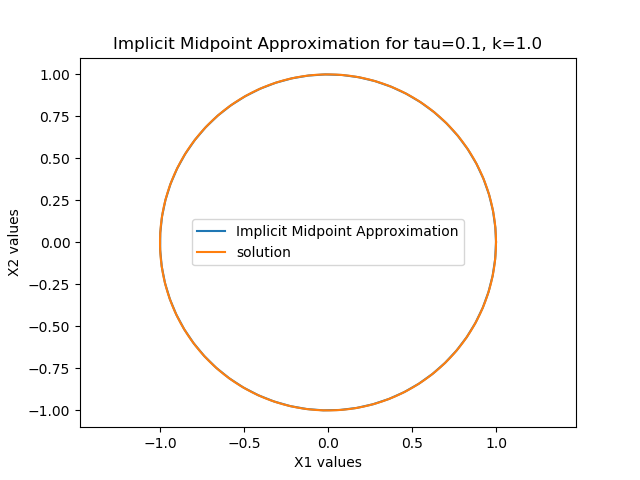
\includegraphics[scale=0.6]{harmonic_phase_mid_01}
		\end{figure}
		As the error is relatively smal, we also provide the
		courser phase graph with stepsize $\tau=0.5$ to beter see the
		difference between the solution and the approximation:
		\begin{figure}[H]
			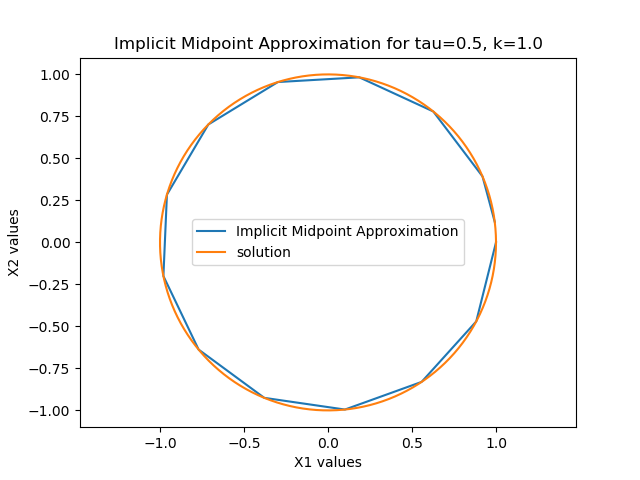
\includegraphics[scale=0.6]{harmonic_phase_mid_05}
		\end{figure}
		As expected, the norm of each estimation point appears to be the
		same as the norm of the initial value.

		We reassert the order of the estimation by displaying the
		log-log graph for the local and the global errors.
		\begin{figure}[H]
			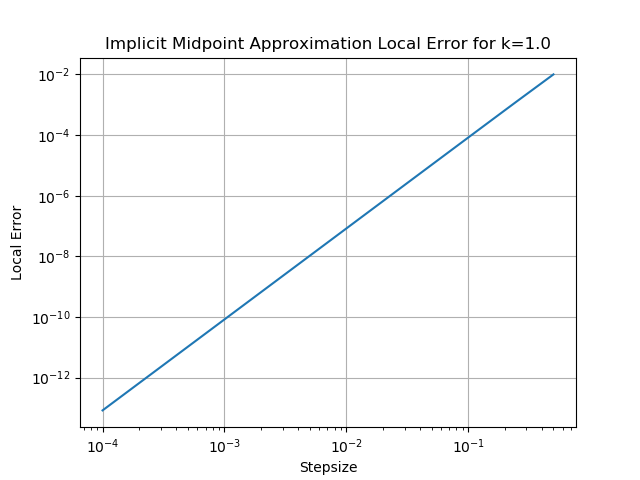
\includegraphics[scale=0.6]{harmonic_mid_local_error}
		\end{figure}
		\begin{figure}[H]
			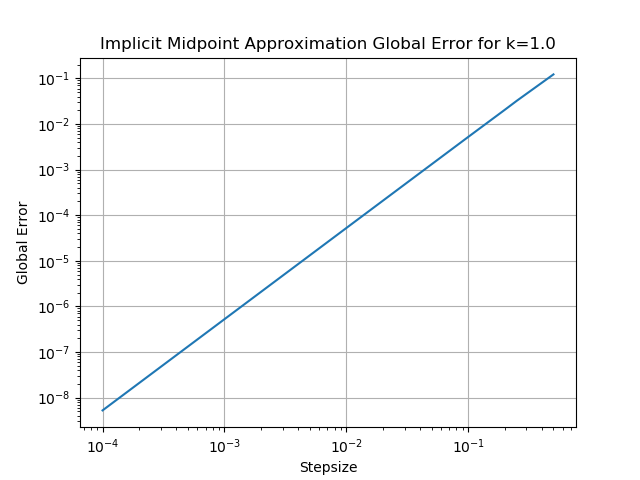
\includegraphics[scale=0.6]{harmonic_mid_global_error}
		\end{figure}
		As expected, the local error graph has a gradient of $3$ and the
		global error graph has a gradient of $2$, as expected for an
		approximation of order $2$.

		For the implicit gauss rk method, we use the formula given by
		Lemma $4.38$
		\[
			R(z) = 1 + z \mathbf{b}^T(I - zA)^{-1} \mathbf{e}
		\]
		to determine stability function.  This is made easier with the
		inverse formula for $2 \times 2$-matrices:
		\[
			\begin{bmatrix}
				a & b \\
				c & d
			\end{bmatrix}^{-1} =
			\frac{1}{ad - bc}
			\begin{bmatrix}
				d & -b \\
				-c & a
			\end{bmatrix}
		\]
		This then gives us the stability function
		\[
			R(z) = \frac{z^2 + 6z + 12}{z^2 - 6z + 12}
		\]
		which is clearly a reversible rational function.  So, from
		Theorem $4.28$, we expect an
		implicit Gauss approximation to be an isometry for any
		stepsize $\tau \in \mathbb{R}$.
		The first terms of the Taylor expansion of $R(z)$ is
		\[
			R(z) = 1 + z^2 + \frac{z^3}{6} + \frac{z^4}{24} +
				\frac{z^5}{144} - \frac{z^6}{1728} \ldots
		\]
		which agrees with the taylor expansion of $e^z$ until the
		$\frac{z^4}{24}$ term.  This confirms that this method is of
		order $4$.

		For a stepsize of $\tau=0.1$,
		the implicit Gauss approximation gives the following
		phase graph:
		\begin{figure}[H]
			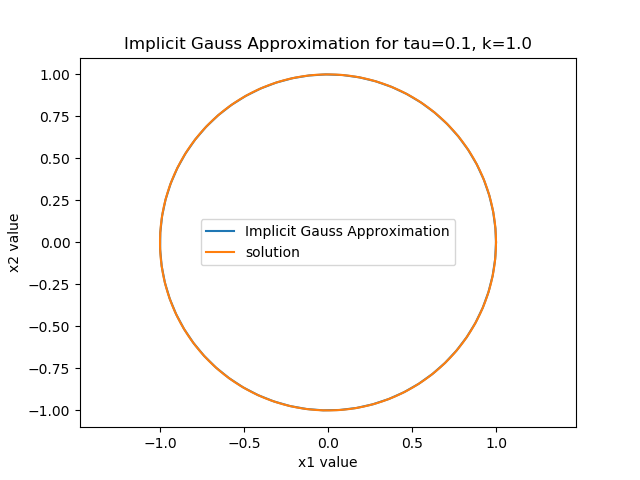
\includegraphics[scale=0.6]{harmonic_phase_gaus_01}
		\end{figure}
		As the error is relatively small, we also provide the
		courser phase graph with stepsize $\tau=0.5$ to beter see the
		difference between the solution and the approximation:
		\begin{figure}[H]
			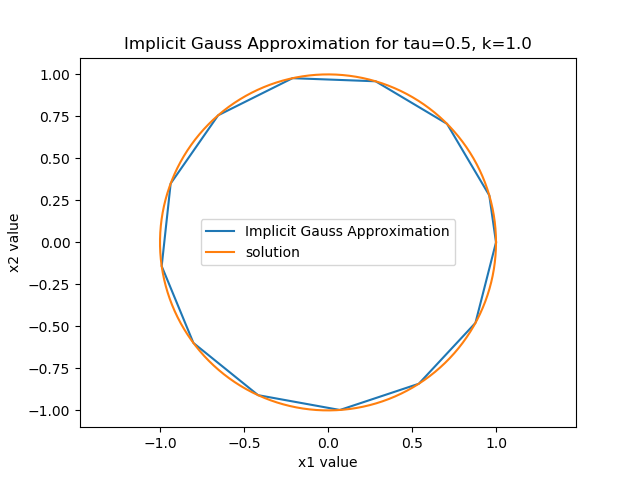
\includegraphics[scale=0.6]{harmonic_phase_gaus_05}
		\end{figure}
		As expected, the norm of each estimation point appears to be the
		same as the norm of the initial value.

		We reassert the order of the estimation by displaying the
		log-log graph for the local and the global errors.
		\begin{figure}[H]
			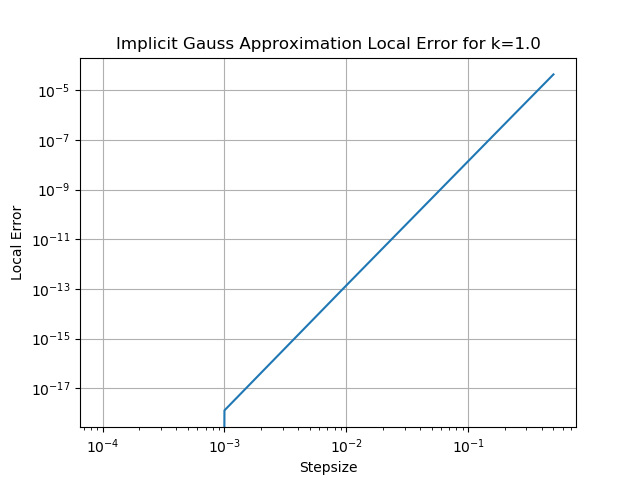
\includegraphics[scale=0.6]{harmonic_gauss_local_error}
		\end{figure}
		\begin{figure}[H]
			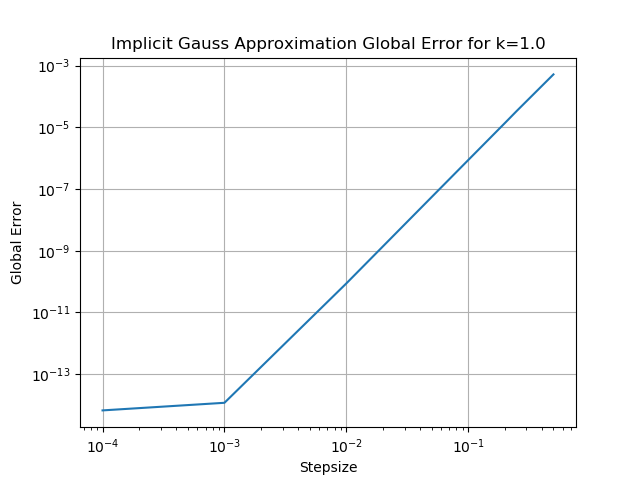
\includegraphics[scale=0.6]{harmonic_gauss_global_error}
		\end{figure}
		We notice that for very small step size, the global error leaves
		the line.  This is most likely due to the error introduced by
		the Newton Method's tolerance allowed.  The local error seems
		for very small values of $\tau$ to get an error so small, that
		the computer is unable to represent it in memory.  This does not
		mean that the estimation is perfect.

		As expected, the local error graph has a gradient of $5$ and the
		global error graph has a gradient of $4$, as expected for an
		approximation of order $4$.

		The eighenvalues of $A=\begin{bmatrix}0 & 1 \\ -1 &
		0\end{bmatrix}$ is $i$ and $-i$. The stability domains of the
		classical explicit Runge-kutta methods of order $3$ and $4$
		contains at least the values $\lambda i, \lambda \in [-1.5,
		1.5]$, therefore our stepsize for the isometric harmonic
		oscillator may be taken as large as $\tau = 1.5$

		The phase graph for the classical Runge Kutta Method of order
		$3$ with stepsize $\tau = 1.5$ give us the following graph.
		\begin{figure}[H]
			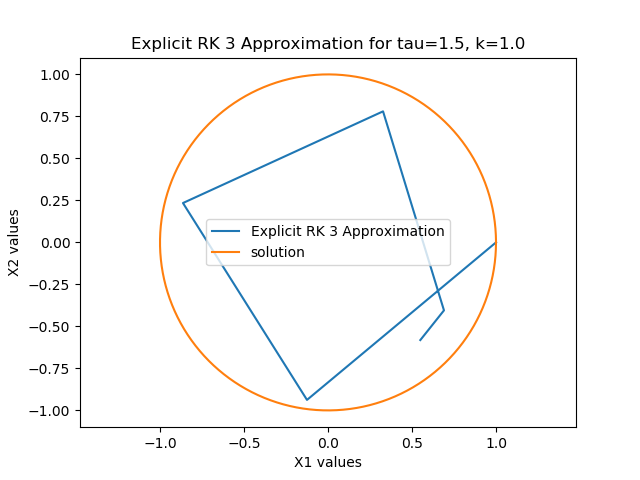
\includegraphics[scale=0.6]{harmonic_phase_erk3_15}
		\end{figure}
		As expected, this is not an isometry, as the vector norm gets
		smaller with every step.
\end{itemize}


\subsection{}
\begin{itemize}
	\item[(a)]
\end{itemize}
\end{document}
